\documentclass[11pt]{beamer}\usepackage[]{graphicx}\usepackage[]{color}
%% maxwidth is the original width if it is less than linewidth
%% otherwise use linewidth (to make sure the graphics do not exceed the margin)
\makeatletter
\def\maxwidth{ %
  \ifdim\Gin@nat@width>\linewidth
    \linewidth
  \else
    \Gin@nat@width
  \fi
}
\makeatother

\definecolor{fgcolor}{rgb}{0.345, 0.345, 0.345}
\newcommand{\hlnum}[1]{\textcolor[rgb]{0.686,0.059,0.569}{#1}}%
\newcommand{\hlstr}[1]{\textcolor[rgb]{0.192,0.494,0.8}{#1}}%
\newcommand{\hlcom}[1]{\textcolor[rgb]{0.678,0.584,0.686}{\textit{#1}}}%
\newcommand{\hlopt}[1]{\textcolor[rgb]{0,0,0}{#1}}%
\newcommand{\hlstd}[1]{\textcolor[rgb]{0.345,0.345,0.345}{#1}}%
\newcommand{\hlkwa}[1]{\textcolor[rgb]{0.161,0.373,0.58}{\textbf{#1}}}%
\newcommand{\hlkwb}[1]{\textcolor[rgb]{0.69,0.353,0.396}{#1}}%
\newcommand{\hlkwc}[1]{\textcolor[rgb]{0.333,0.667,0.333}{#1}}%
\newcommand{\hlkwd}[1]{\textcolor[rgb]{0.737,0.353,0.396}{\textbf{#1}}}%

\usepackage{framed}
\makeatletter
\newenvironment{kframe}{%
 \def\at@end@of@kframe{}%
 \ifinner\ifhmode%
  \def\at@end@of@kframe{\end{minipage}}%
  \begin{minipage}{\columnwidth}%
 \fi\fi%
 \def\FrameCommand##1{\hskip\@totalleftmargin \hskip-\fboxsep
 \colorbox{shadecolor}{##1}\hskip-\fboxsep
     % There is no \\@totalrightmargin, so:
     \hskip-\linewidth \hskip-\@totalleftmargin \hskip\columnwidth}%
 \MakeFramed {\advance\hsize-\width
   \@totalleftmargin\z@ \linewidth\hsize
   \@setminipage}}%
 {\par\unskip\endMakeFramed%
 \at@end@of@kframe}
\makeatother

\definecolor{shadecolor}{rgb}{.97, .97, .97}
\definecolor{messagecolor}{rgb}{0, 0, 0}
\definecolor{warningcolor}{rgb}{1, 0, 1}
\definecolor{errorcolor}{rgb}{1, 0, 0}
\newenvironment{knitrout}{}{} % an empty environment to be redefined in TeX

\usepackage{alltt}
\usetheme{Warsaw}
\usepackage[utf8]{inputenc}
\usepackage{amsmath}
\usepackage{amsfonts}
\usepackage{amssymb}
\usepackage{array}
\usepackage{graphicx}
\author{John Muschelli}
\usepackage{hyperref}
\usepackage{tikz}
\usetikzlibrary{calc,intersections}

\usetikzlibrary{shapes,arrows}
\usetikzlibrary{positioning}
\setbeamertemplate{navigation symbols}{}%remove navigation symbols

\title{Image Processing with fslr}
%\setbeamercovered{transparent} 
%\setbeamertemplate{navigation symbols}{} 
%\logo{} 
\institute{Johns Hopkins Bloomberg School of Public Health} 
%\date{} 
%\subject{} 
\setlength{\topsep}{0pt}
\setlength{\parskip}{0pt}
\setlength{\partopsep}{1pt}
\setbeamertemplate{footline}[frame number]

\usepackage[
  natbib = true,
    backend=bibtex,
]{biblatex}
\bibliography{fslr_reg}
\AtEveryBibitem{
\clearfield{note}
% \clearlist{address}
% \clearfield{eprint}
% \clearfield{isbn}
% \clearfield{issn}
% \clearlist{location}
% \clearfield{month}
% \clearfield{series}
} % clears language


\newcommand {\framedgraphic}[2] {
    \begin{frame}{#1}
        \begin{center}
            \includegraphics[width=\textwidth,height=0.8\textheight,keepaspectratio]{#2}
        \end{center}
    \end{frame}
}
\IfFileExists{upquote.sty}{\usepackage{upquote}}{}
\begin{document}

\begin{frame}
\titlepage
\end{frame}

%\begin{frame}
%\tableofcontents
%\end{frame}




\begin{frame}[fragile]{FSL and fslr}

\begin{itemize}
\item FSL is a comprehensive library of analysis tools for fMRI, MRI and DTI brain imaging data. 
	\begin{itemize}
	\item Collection of routines in C, C++
	\end{itemize}
\item fslr: port of FSL into R
\item The two functions we focus on are: 
\begin{enumerate}
\item Image inhomogeneity correction (using FAST \citep{zhang2001segmentation})
\item Image registration
\end{enumerate} 
\end{itemize}

\end{frame}


\begin{frame}[fragile]{Installing fslr}
First, you must Install FSL \href{http://fsl.fmrib.ox.ac.uk/fsl/fslwiki/FslInstallation}{http://fsl.fmrib.ox.ac.uk/fsl/fslwiki/FslInstallation}.  \\
\vspace{0.5cm}
\verb|fslr| is installed on CRAN, but the development arm of \verb|fslr| is most likely the best to install, using the \verb|devtools| package:

\begin{knitrout}
\definecolor{shadecolor}{rgb}{0.969, 0.969, 0.969}\color{fgcolor}\begin{kframe}
\begin{alltt}
\hlkwa{if} \hlstd{(}\hlopt{!}\hlkwd{require}\hlstd{(devtools))\{}
        \hlkwd{install.packages}\hlstd{(}\hlstr{'devtools'}\hlstd{)}
\hlstd{\}}
\hlstd{devtools}\hlopt{::}\hlkwd{install_github}\hlstd{(}\hlstr{"muschellij2/fslr"}\hlstd{)}
\end{alltt}
\end{kframe}
\end{knitrout}
\end{frame}

\begin{frame}[fragile]{Structure of fslr functions}


\tikzstyle{bblock} = [rectangle, draw, text width=7em, text centered, minimum height=2em, rounded corners, align=flush center]
\tikzstyle{line} = [draw, text centered , -latex']
\tikzstyle{line node} = [draw, fill=white, font=\tiny ]
\tikzstyle{block} = [rectangle, draw, text width=5em, text centered, minimum height=4em, rounded corners]    


\begin{figure}
\centering
\begin{tikzpicture}[node distance = .5cm, every node/.style={rectangle,fill=white},  transform shape]
% Place nodes
\node [bblock] (fname) {Character filename};
%\node [bblock, right=1cm of fname] (nim) {\verb|nifti| object};
\node [bblock, below right=1cm and 0.1cm of fname] (fslr_func) {fslr function (call FSL function) };
%\node [bblock, above right=1cm and 0.1cm of fslr_func] (nim) {nifti object in R };
\node [bblock, right=3cm of fname] (nim) {nifti object in R };
\node [bblock, below left=1cm and 0.1cm of fslr_func] (nii_back) { Return nifti object to R };
\node [bblock, right=3cm of nii_back] (write) { Write Image to Disk };


% Draw edges
%\path [line] (nim) -| node[xshift=-0.1cm] {} ([xshift=.1 cm]fslr_func.north);
%\path [line] (fname) -| node[xshift=0.1cm] {or} ([xshift=-.1 cm]fslr_func.north);
\path [line] (nim) -| node {} (fslr_func.north);
\path [line] (fname) -| node {or} (fslr_func.north);
%\path [line] (fname) -| ([xshift=-.1 cm]fslr_func.north);
\path [line] ([xshift=.1 cm]fslr_func.south) |- node[xshift=0.1cm] {} (write);
\path [line] ([xshift=-.1 cm]fslr_func.south) |- node[xshift=0.1cm] {and/or} (nii_back);
%\path [line] ([xshift=-.1 cm]fslr_func.south) |- (nii_back);
%\path [line] (fslr_func) |- (write);
%\coordinate[xshift=0.1 cm] (fslr_func) at (write);
%\path [line] (fslr_func) |- (write)+(0,0.1 cm);

\end{tikzpicture}
\end{figure}

\end{frame}


\begin{frame}[fragile]{Interactive/GUI vs. Terminal R}

In general, GUI-based apps do not inherit the shell environment (aka if \verb|FSLDIR| is defined in your Terminal, RStudio doesn't see it).

For fslr to work, it must know where the directory FSL was installed.  If \verb|FSLDIR| is found, it will be used.  You can check this by 2 ways:

\begin{knitrout}
\definecolor{shadecolor}{rgb}{0.969, 0.969, 0.969}\color{fgcolor}\begin{kframe}
\begin{alltt}
\hlkwd{Sys.getenv}\hlstd{(}\hlstr{"FSLDIR"}\hlstd{)}
\end{alltt}
\begin{verbatim}
[1] ""
\end{verbatim}
\begin{alltt}
\hlkwd{library}\hlstd{(fslr)}
\hlkwd{have.fsl}\hlstd{()}
\end{alltt}
\begin{verbatim}
[1] TRUE
\end{verbatim}
\end{kframe}
\end{knitrout}

If \verb|have.fsl()= FALSE| then you must specify the path using:

\begin{knitrout}
\definecolor{shadecolor}{rgb}{0.969, 0.969, 0.969}\color{fgcolor}\begin{kframe}
\begin{alltt}
\hlkwd{options}\hlstd{(}\hlkwc{fsl.path}\hlstd{=}\hlstr{"/my/path/to/fsl"}\hlstd{)}
\end{alltt}
\end{kframe}
\end{knitrout}



\end{frame}


\begin{frame}[fragile]{fslmaths: Math with FSL}
\verb|fslmaths| (in fslr) calls \verb|fslmaths| from FSL (see \verb|fslr::fslmaths.help()| for help):
Let's read an image in using \verb|readNIfTI| from \verb|oro.nifti|:

\begin{knitrout}
\definecolor{shadecolor}{rgb}{0.969, 0.969, 0.969}\color{fgcolor}\begin{kframe}
\begin{alltt}
\hlkwd{library}\hlstd{(oro.nifti)}
\hlstd{t1_fname} \hlkwb{=} \hlstr{"~/Neurohacking_data/BRAINIX/NIfTI/T1.nii.gz"}
\hlstd{nim} \hlkwb{=} \hlkwd{readNIfTI}\hlstd{(t1_fname,} \hlkwc{reorient}\hlstd{=}\hlnum{FALSE}\hlstd{)}
\end{alltt}
\end{kframe}
\end{knitrout}
\end{frame}

\begin{frame}[fragile]{fslstats: Stats with FSL}
\verb|fslstats| (in fslr) calls \verb|fslstats| from FSL (see \verb|fslr::fslstats.help()| for help):

We can do statistics (e.g.~mean) in R and fslr:
\begin{knitrout}
\definecolor{shadecolor}{rgb}{0.969, 0.969, 0.969}\color{fgcolor}\begin{kframe}
\begin{alltt}
\hlkwd{mean}\hlstd{(nim)}
\end{alltt}
\begin{verbatim}
[1] 102.4701
\end{verbatim}
\begin{alltt}
\hlkwd{fslstats}\hlstd{(nim,} \hlkwc{opts}\hlstd{=}\hlstr{"-m"}\hlstd{)}
\end{alltt}
\begin{verbatim}
[1] "102.470113"
\end{verbatim}
\begin{alltt}
\hlkwd{fslstats}\hlstd{(}\hlstr{"Output_3D_File.nii.gz"}\hlstd{,} \hlkwc{opts} \hlstd{=} \hlstr{"-m"}\hlstd{)}
\end{alltt}
\begin{verbatim}
[1] "102.470113"
\end{verbatim}
\end{kframe}
\end{knitrout}


\end{frame}


\begin{frame}[fragile]{fslr: Bias Field Correction}

\verb|fslr::fsl_biascorrect| calls \verb|fast| from FSL which incorporates the bias field correction by \citet{guillemaud1997estimating}:

\begin{knitrout}
\definecolor{shadecolor}{rgb}{0.969, 0.969, 0.969}\color{fgcolor}\begin{kframe}
\begin{alltt}
\hlstd{fast_img} \hlkwb{=} \hlkwd{fsl_biascorrect}\hlstd{(nim,}
        \hlkwc{retimg}\hlstd{=}\hlnum{TRUE}\hlstd{)}
\end{alltt}
\begin{verbatim}
FSLDIR='/usr/local/fsl'; export FSLDIR; sh "${FSLDIR}/etc/fslconf/fsl.sh"; FSLOUTPUTTYPE=NIFTI_GZ; export FSLOUTPUTTYPE; $FSLDIR/bin/fast    -B --nopve --out="/var/folders/1s/wrtqcpxn685_zk570bnx9_rr0000gr/T//Rtmpu1bWFr/file36472b611ed9" "/var/folders/1s/wrtqcpxn685_zk570bnx9_rr0000gr/T//Rtmpu1bWFr/file3647404bb909.nii.gz"; 
\end{verbatim}
\end{kframe}
\end{knitrout}
\end{frame}



\begin{frame}[fragile]{fslr: Bias Field Correction}

\begin{tabular}{cc}
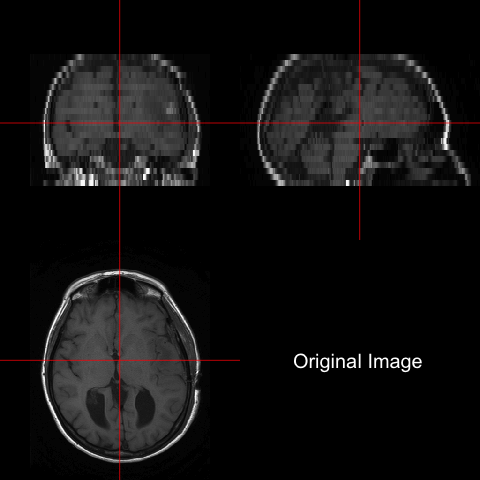
\includegraphics[width=0.5\linewidth]{Orig_Image.png} & 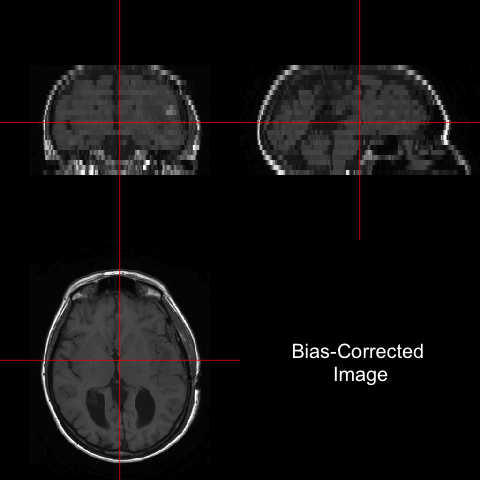
\includegraphics[width=0.5\linewidth]{FAST_Image.png}
\end{tabular}

\end{frame}


\begin{frame}[fragile]{fslr: Bias Field Correction - Difference Image}

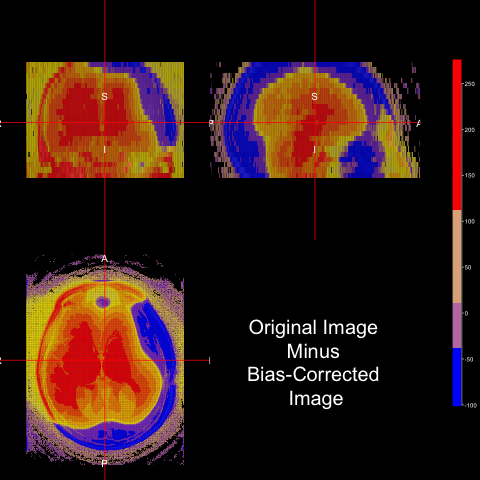
\includegraphics[width=0.5\linewidth]{FAST_Diff_Image.png}

\end{frame}


\begin{knitrout}
\definecolor{shadecolor}{rgb}{0.969, 0.969, 0.969}\color{fgcolor}
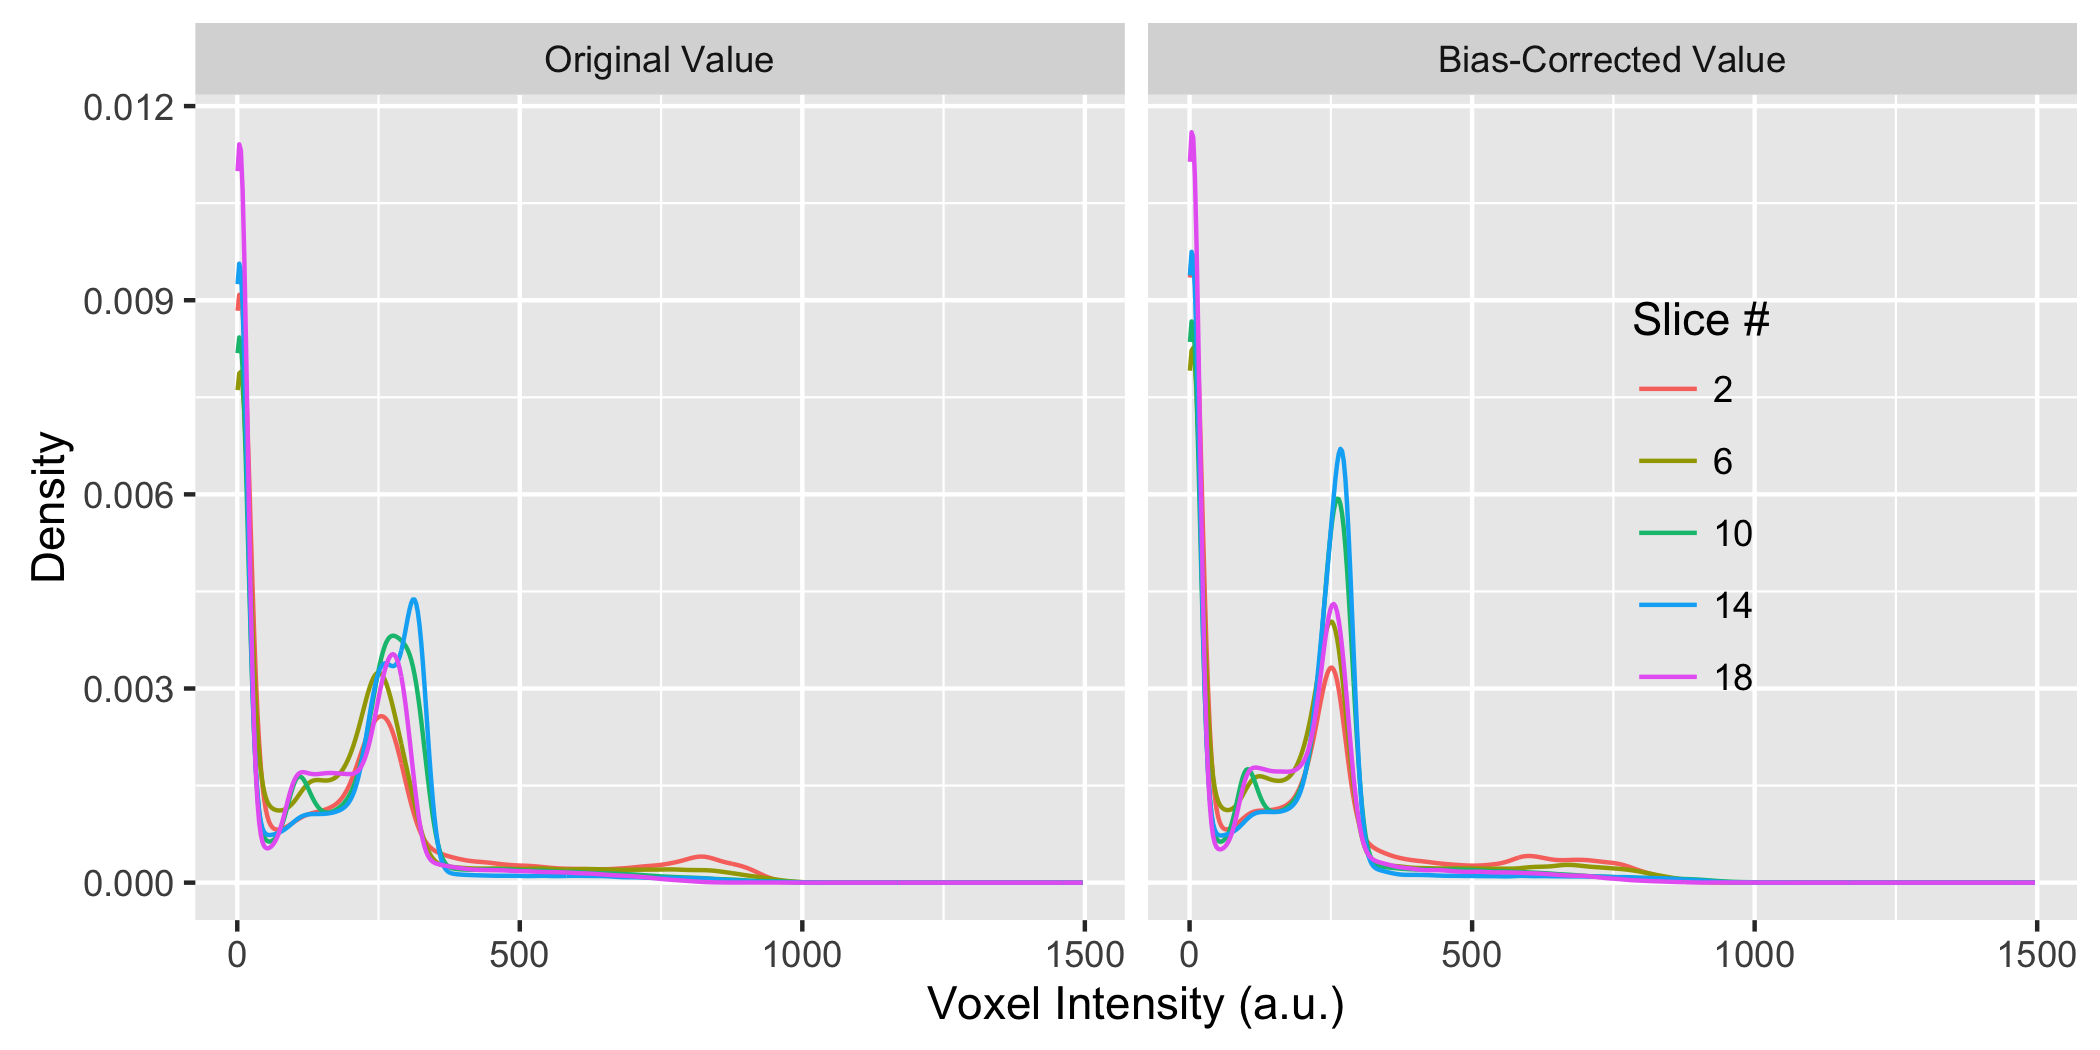
\includegraphics[width=\textwidth,height=0.5\textheight,keepaspectratio]{figure/hist_plot_n4-1} 

\end{knitrout}


\begin{frame}[fragile]{fslr: Bias Field Correction - Hists}

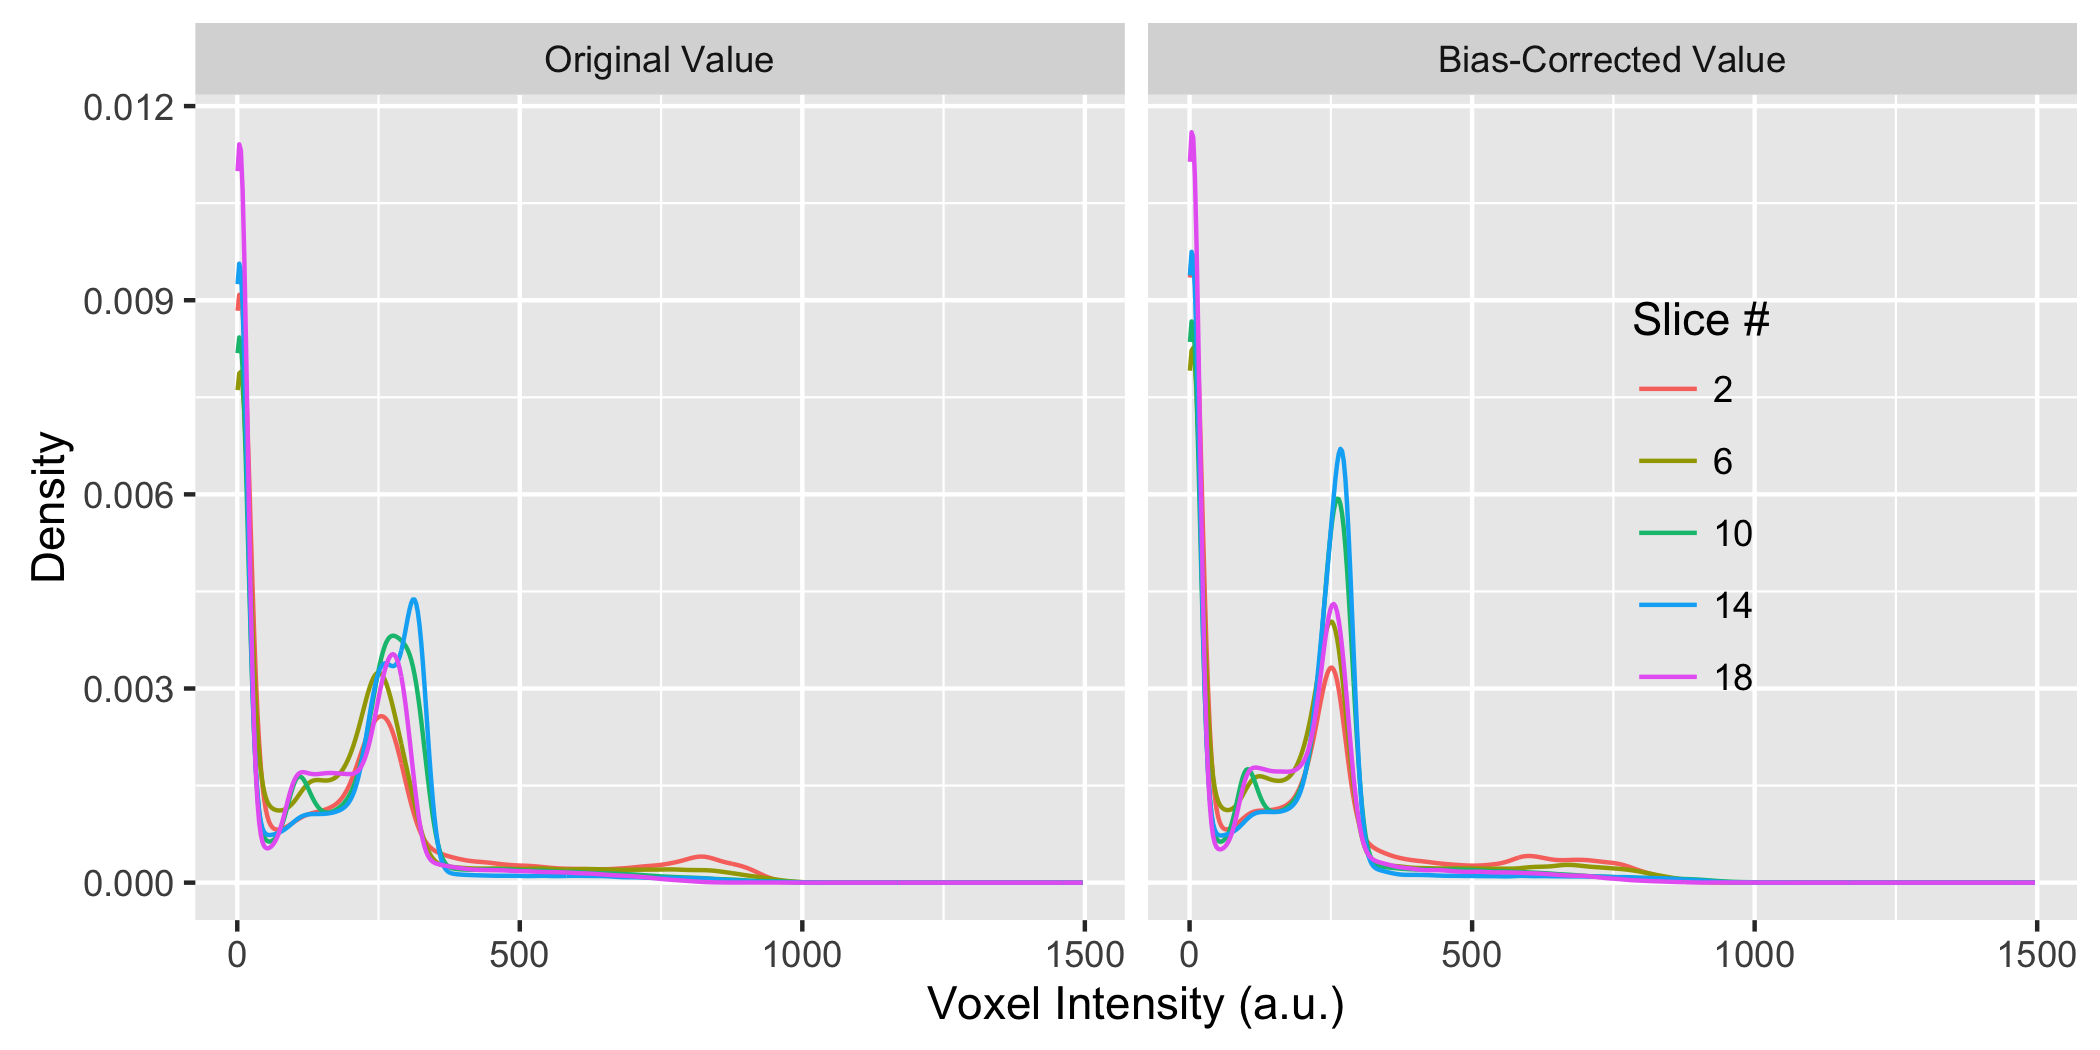
\includegraphics[width=\linewidth]{figure/hist_plot_n4-1.png}


\end{frame}



\begin{frame}[fragile]{ANTsR: Bias Field Correction}

We use the bias\_correct function in extrantsr to do an inhomogeneity correction (N3 or N4) for  the T1w image.  Here we will do N4 inhomogeneity correction:

\begin{knitrout}
\definecolor{shadecolor}{rgb}{0.969, 0.969, 0.969}\color{fgcolor}\begin{kframe}
\begin{alltt}
\hlkwd{library}\hlstd{(extrantsr)}
\hlstd{n4_img} \hlkwb{=} \hlkwd{bias_correct}\hlstd{(nim,}
                      \hlkwc{correction} \hlstd{=} \hlstr{"N4"}\hlstd{,}
                      \hlkwc{retimg}\hlstd{=}\hlnum{TRUE}\hlstd{)}
\end{alltt}
\end{kframe}
\end{knitrout}
\end{frame}



\begin{frame}[fragile]{ANTsR: Bias Field Correction}

\begin{tabular}{cc}
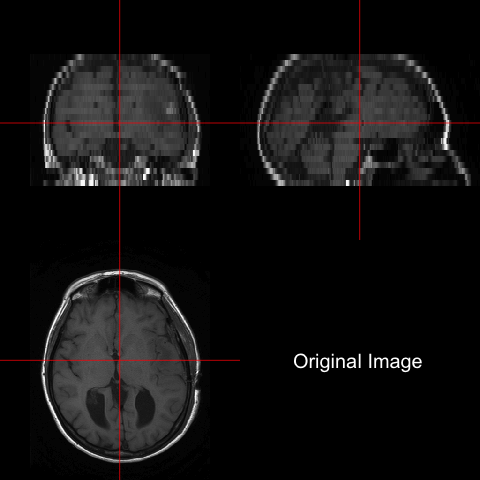
\includegraphics[width=0.5\linewidth]{Orig_Image.png} & 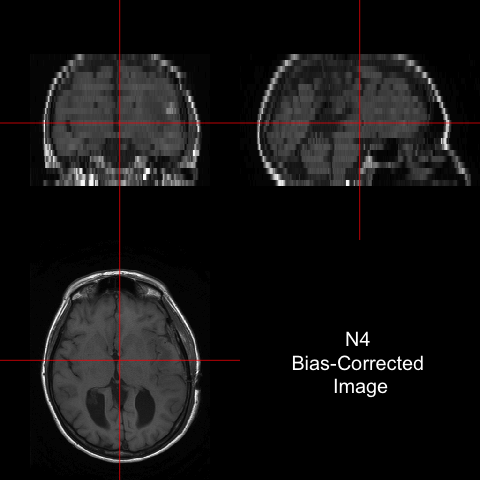
\includegraphics[width=0.5\linewidth]{N4_Image.png}
\end{tabular}

\end{frame}


\begin{frame}[fragile]{fslr: Bias Field Correction - Difference Iage}

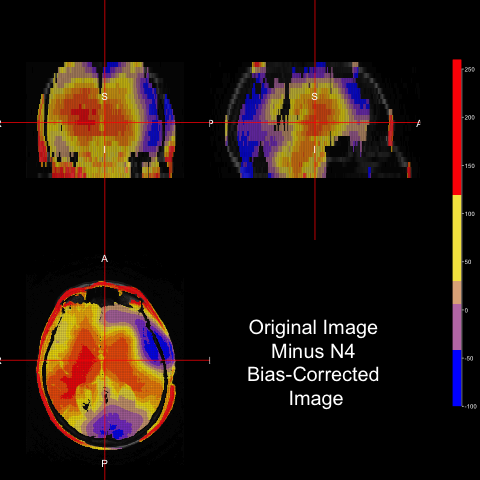
\includegraphics[width=0.5\linewidth]{N4_Diff_Image.png}

\end{frame}



\begin{frame}[fragile]{fslr: Brain Extraction}

FSL's Brain Extraction Tool (BET) can be used for skull stripping.  It is fast, robust, and one of the most popular for this task.  \verb|fslr::fslbet| is used to call the FSL commands \verb|bet2|, which does brain extraction or \verb|bet|, which does brain extraction with additional options.

\begin{knitrout}
\definecolor{shadecolor}{rgb}{0.969, 0.969, 0.969}\color{fgcolor}\begin{kframe}
\begin{alltt}
\hlstd{bet_fast} \hlkwb{=} \hlkwd{fslbet}\hlstd{(}\hlkwc{infile}\hlstd{=fast_img,} \hlkwc{retimg}\hlstd{=}\hlnum{TRUE}\hlstd{)}
\end{alltt}
\begin{verbatim}
FSLDIR='/usr/local/fsl'; export FSLDIR; sh "${FSLDIR}/etc/fslconf/fsl.sh"; FSLOUTPUTTYPE=NIFTI_GZ; export FSLOUTPUTTYPE; $FSLDIR/bin/bet2 "/var/folders/1s/wrtqcpxn685_zk570bnx9_rr0000gr/T//RtmpuK0Ep8/file712310f4319d.nii.gz" "/var/folders/1s/wrtqcpxn685_zk570bnx9_rr0000gr/T//RtmpuK0Ep8/file7123398dde28"  
\end{verbatim}
\end{kframe}
\end{knitrout}
\end{frame}




\begin{frame}[fragile]{fslr: Brain Extraction Results}

\begin{tabular}{cc}
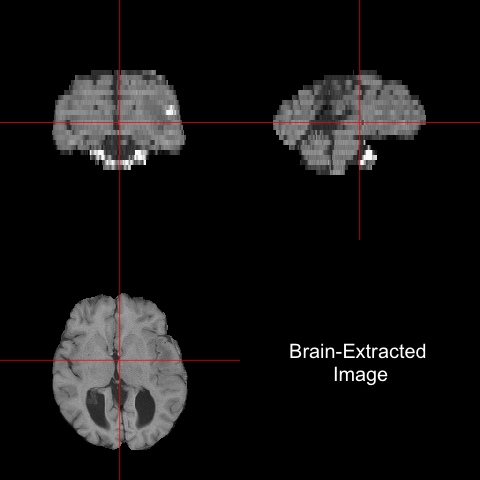
\includegraphics[width=0.5\linewidth]{BET_Image.png} & 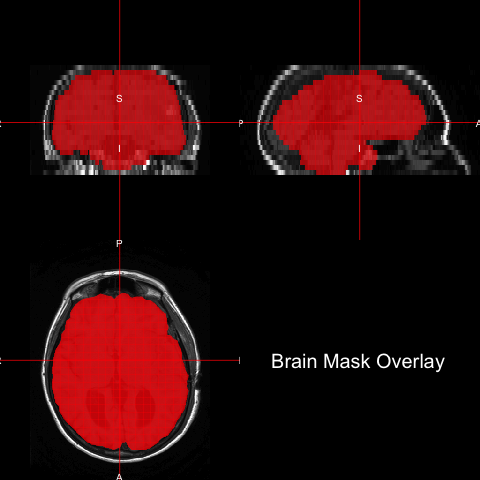
\includegraphics[width=0.5\linewidth]{BET_Image_Overlay.png}
\end{tabular}

\end{frame}


\begin{frame}[fragile]{fslr: Better Brain Extraction}

There are some parts of the brain not segmented in the image.  We can estimate the center of gravity (COG) from the brain extracted image, and then re-run bet with the new COG to get a better result

\begin{knitrout}
\definecolor{shadecolor}{rgb}{0.969, 0.969, 0.969}\color{fgcolor}\begin{kframe}
\begin{alltt}
\hlstd{cog} \hlkwb{=} \hlkwd{cog}\hlstd{(bet_fast,} \hlkwc{ceil}\hlstd{=}\hlnum{TRUE}\hlstd{)}
\hlstd{cog} \hlkwb{=} \hlkwd{paste}\hlstd{(}\hlstr{"-c"}\hlstd{,} \hlkwd{paste}\hlstd{(cog,}
                        \hlkwc{collapse}\hlstd{=} \hlstr{" "}\hlstd{))}
\hlstd{bet_fast2} \hlkwb{=} \hlkwd{fslbet}\hlstd{(}\hlkwc{infile}\hlstd{=fast_img,} \hlkwc{retimg}\hlstd{=}\hlnum{TRUE}\hlstd{,}
                   \hlkwc{opts} \hlstd{= cog)}
\end{alltt}
\begin{verbatim}
FSLDIR='/usr/local/fsl'; export FSLDIR; sh "${FSLDIR}/etc/fslconf/fsl.sh"; FSLOUTPUTTYPE=NIFTI_GZ; export FSLOUTPUTTYPE; $FSLDIR/bin/bet2 "/private/var/folders/1s/wrtqcpxn685_zk570bnx9_rr0000gr/T/Rtmp6LNVs4/file14e4639409ef9.nii.gz" "/var/folders/1s/wrtqcpxn685_zk570bnx9_rr0000gr/T//Rtmp6LNVs4/file14e46342e04da" -c 258 222 12 
\end{verbatim}
\end{kframe}
\end{knitrout}
\end{frame}



\begin{frame}[fragile]{fslr: Better Brain Extraction Results}

\begin{tabular}{cc}
Before COG & After COG \\
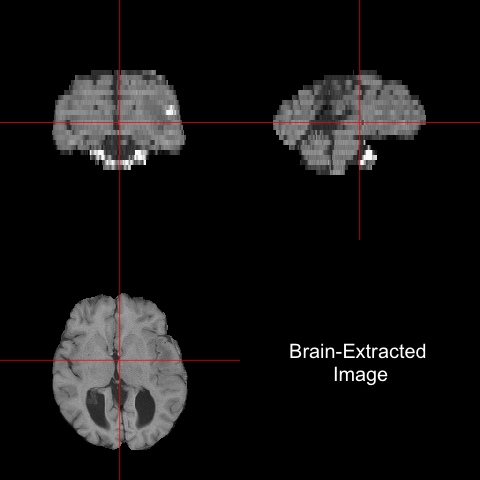
\includegraphics[width=0.4\linewidth]{BET_Image.png} & 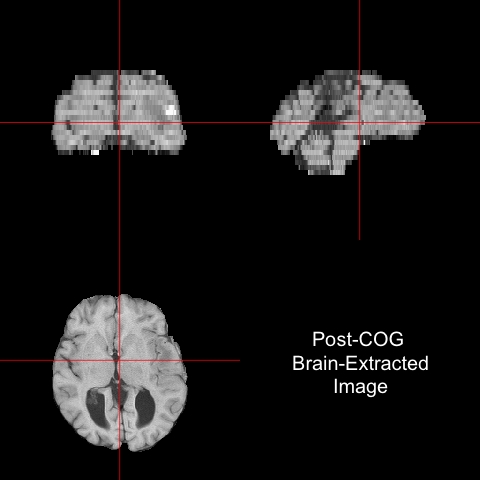
\includegraphics[width=0.4\linewidth]{BET_Image2.png} \\
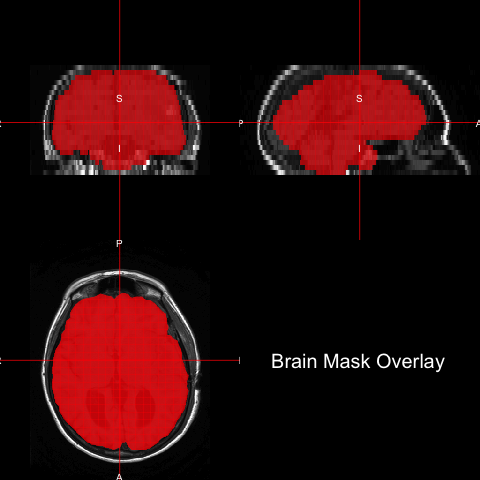
\includegraphics[width=0.4\linewidth]{BET_Image_Overlay.png} & 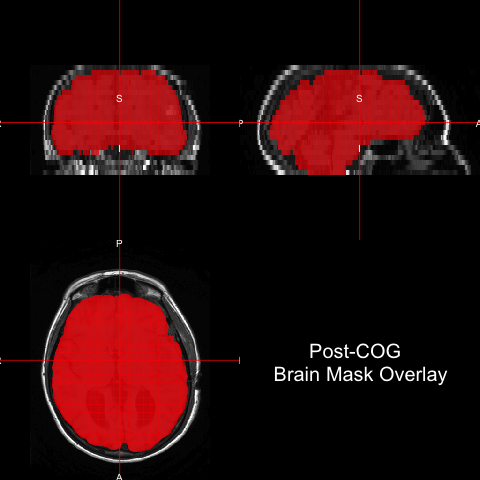
\includegraphics[width=0.4\linewidth]{BET_Image_Overlay2.png}
\end{tabular}

\end{frame}

\begin{frame}[fragile]{fslr: Image Registration (Linear)}

From FSL: ``FLIRT (FMRIB's Linear Image Registration Tool) is a fully automated robust and accurate tool for linear (affine) intra- and inter-modal brain image registration''

\verb|fslr::flirt| takes in a input filename (or nifti) and a reference filename (or nifti) to transform the infile to:
\begin{knitrout}
\definecolor{shadecolor}{rgb}{0.969, 0.969, 0.969}\color{fgcolor}\begin{kframe}
\begin{alltt}
\hlstd{registered_fast} \hlkwb{=} \hlkwd{flirt}\hlstd{(}\hlkwc{infile}\hlstd{=fast_img,}
        \hlkwc{reffile} \hlstd{=} \hlstr{"MNI152_T1_1mm.nii.gz"}\hlstd{,}
        \hlkwc{dof} \hlstd{=} \hlnum{6}\hlstd{,}
        \hlkwc{retimg} \hlstd{=} \hlnum{TRUE}\hlstd{)}
\end{alltt}
\begin{verbatim}
FSLDIR='/usr/local/fsl'; export FSLDIR; sh "${FSLDIR}/etc/fslconf/fsl.sh"; FSLOUTPUTTYPE=NIFTI_GZ; export FSLOUTPUTTYPE; $FSLDIR/bin/flirt -in "/var/folders/1s/wrtqcpxn685_zk570bnx9_rr0000gr/T//RtmpmZyFeZ/file5c6273a91b69.nii.gz" -ref "MNI152_T1_1mm.nii.gz" -out "/var/folders/1s/wrtqcpxn685_zk570bnx9_rr0000gr/T//RtmpmZyFeZ/file5c62685441c1" -dof 6 -omat "/var/folders/1s/wrtqcpxn685_zk570bnx9_rr0000gr/T//RtmpmZyFeZ/file5c626346c5d1.mat"  
\end{verbatim}
\end{kframe}
\end{knitrout}
\end{frame}




\begin{frame}[fragile]{fslr: Image Registration (Linear) Results}

\begin{tabular}{cc}
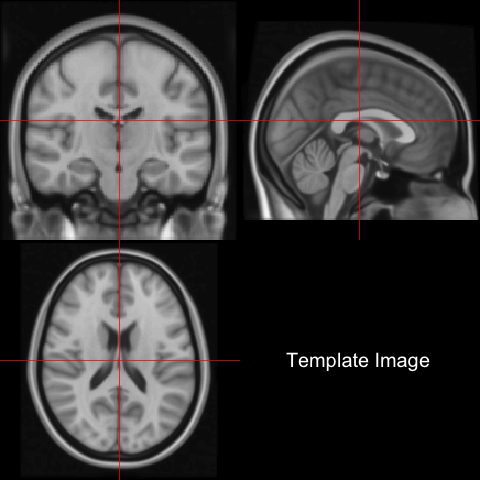
\includegraphics[width=0.5\linewidth]{Template.png} & 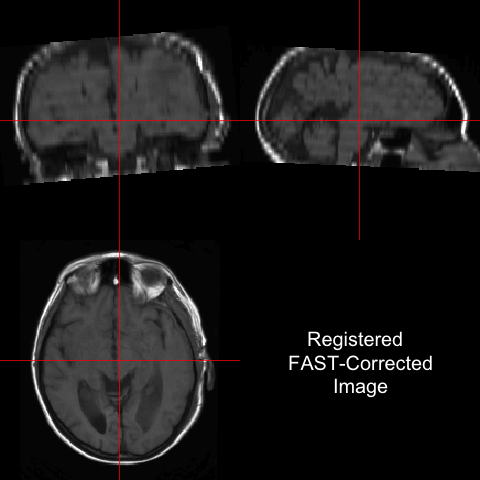
\includegraphics[width=0.5\linewidth]{FLIRT_Reg_Image.png}
\end{tabular}

\end{frame}



\begin{frame}[fragile]{fslr: Image Registration (Linear) Brain}

Let's use linear registration with brains only:
\begin{knitrout}
\definecolor{shadecolor}{rgb}{0.969, 0.969, 0.969}\color{fgcolor}\begin{kframe}
\begin{alltt}
\hlstd{registered_fast_brain} \hlkwb{=} \hlkwd{flirt}\hlstd{(}\hlkwc{infile}\hlstd{=bet_fast2,}
  \hlkwc{reffile} \hlstd{=} \hlstr{"MNI152_T1_1mm_brain.nii.gz"}\hlstd{,}
        \hlkwc{dof} \hlstd{=} \hlnum{6}\hlstd{,}
        \hlkwc{retimg} \hlstd{=} \hlnum{TRUE}\hlstd{)}
\end{alltt}
\begin{verbatim}
FSLDIR='/usr/local/fsl'; export FSLDIR; sh "${FSLDIR}/etc/fslconf/fsl.sh"; FSLOUTPUTTYPE=NIFTI_GZ; export FSLOUTPUTTYPE; $FSLDIR/bin/flirt -in "/var/folders/1s/wrtqcpxn685_zk570bnx9_rr0000gr/T//RtmpRqyJKh/file819f2085a79b.nii.gz" -ref "MNI152_T1_1mm_brain.nii.gz" -out "/var/folders/1s/wrtqcpxn685_zk570bnx9_rr0000gr/T//RtmpRqyJKh/file819f3d68a284" -dof 6 -omat "/var/folders/1s/wrtqcpxn685_zk570bnx9_rr0000gr/T//RtmpRqyJKh/file819f26bec1cb.mat"  
\end{verbatim}
\end{kframe}
\end{knitrout}
\end{frame}




\begin{frame}[fragile]{fslr: Image Registration (Linear) Results}

\begin{tabular}{cc}
\includegraphics[width=0.5\linewidth]{Template_Brain.png} & 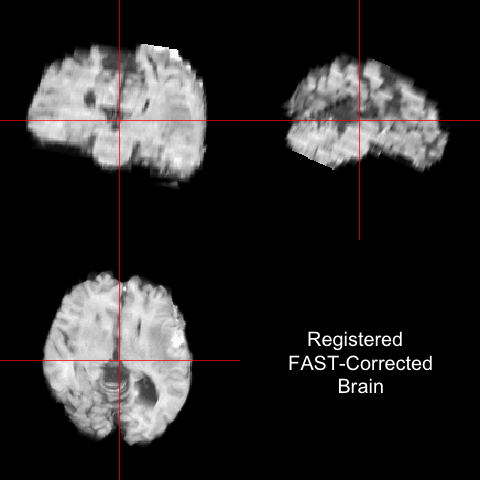
\includegraphics[width=0.5\linewidth]{FLIRT_Reg_Image_Brain.png}
\end{tabular}

\end{frame}

\begin{knitrout}
\definecolor{shadecolor}{rgb}{0.969, 0.969, 0.969}\color{fgcolor}\begin{kframe}
\begin{verbatim}
FSLDIR='/usr/local/fsl'; export FSLDIR; sh "${FSLDIR}/etc/fslconf/fsl.sh"; FSLOUTPUTTYPE=NIFTI_GZ; export FSLOUTPUTTYPE; $FSLDIR/bin/flirt -in "/var/folders/1s/wrtqcpxn685_zk570bnx9_rr0000gr/T//Rtmp4iTpSa/file7e3a619ccf8f.nii.gz" -ref "MNI152_T1_1mm_brain.nii.gz" -out "/var/folders/1s/wrtqcpxn685_zk570bnx9_rr0000gr/T//Rtmp4iTpSa/file7e3a2f8d3cf4" -dof 12 -omat "/var/folders/1s/wrtqcpxn685_zk570bnx9_rr0000gr/T//Rtmp4iTpSa/file7e3a7dfee759.mat"  
\end{verbatim}
\end{kframe}
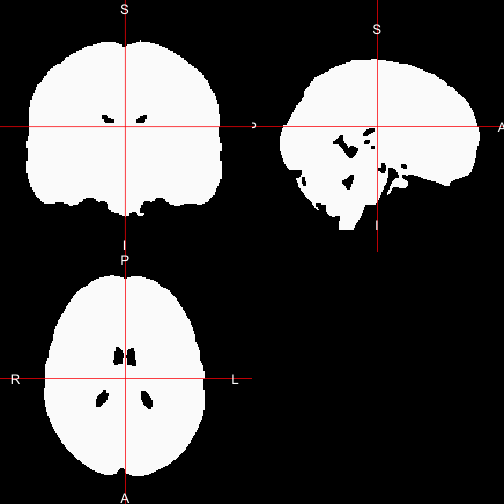
\includegraphics[width=\textwidth,height=0.5\textheight,keepaspectratio]{figure/image_affine_bet-1} 
\begin{kframe}\begin{verbatim}
RStudioGD 
        2 
\end{verbatim}
\end{kframe}
\end{knitrout}

\begin{frame}[fragile]{fslr: Image Registration (Affine) Results}
Instead of a rigid-body registration, let us try an affine (still linear) registration:
\begin{tabular}{cc}
\includegraphics[width=0.5\linewidth]{Template_Brain.png} & 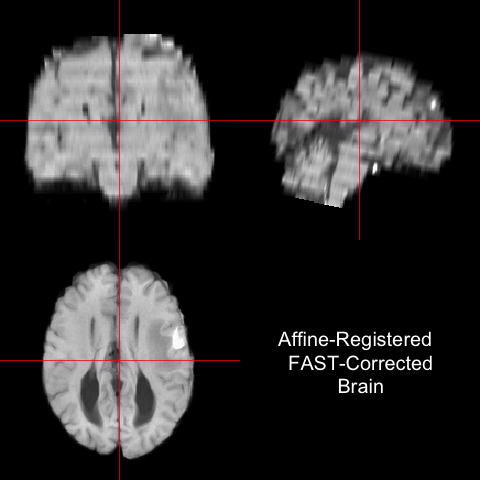
\includegraphics[width=0.5\linewidth]{FLIRT_Affine_Image_Brain.png}
\end{tabular}

\end{frame}


\begin{frame}[fragile]{fslr: Image Registration (Non-Linear)}
FNIRT performs non-linear registration. An affine registration must be performed before using FNIRT.

FLIRT can also do Affine registrations (DOF = 12), and \verb|fslr::fnirt_with_affine| will perform an affine registration than FNIRT.  You want to perform this on skull-stripped images. 


\begin{knitrout}
\definecolor{shadecolor}{rgb}{0.969, 0.969, 0.969}\color{fgcolor}\begin{kframe}
\begin{alltt}
\hlstd{fnirt_fast} \hlkwb{=} \hlkwd{fnirt_with_affine}\hlstd{(}\hlkwc{infile}\hlstd{=bet_fast2,}
        \hlkwc{reffile} \hlstd{=} \hlstr{"MNI152_T1_1mm_brain.nii.gz"}\hlstd{,}
        \hlkwc{outfile} \hlstd{=} \hlstr{"FNIRT_to_Template"}\hlstd{,} \hlkwc{retimg}\hlstd{=}\hlnum{TRUE}\hlstd{)}
\end{alltt}
\begin{verbatim}
FSLDIR='/usr/local/fsl'; export FSLDIR; sh "${FSLDIR}/etc/fslconf/fsl.sh"; FSLOUTPUTTYPE=NIFTI_GZ; export FSLOUTPUTTYPE; $FSLDIR/bin/flirt -in "/var/folders/1s/wrtqcpxn685_zk570bnx9_rr0000gr/T//RtmpUFGTVc/file842e65483fd1.nii.gz" -ref "MNI152_T1_1mm_brain.nii.gz" -out "/var/folders/1s/wrtqcpxn685_zk570bnx9_rr0000gr/T//RtmpUFGTVc/file842e43b800fa" -dof 12 -omat "/var/folders/1s/wrtqcpxn685_zk570bnx9_rr0000gr/T//RtmpUFGTVc/file842e18295d7a"  
FSLDIR='/usr/local/fsl'; export FSLDIR; sh "${FSLDIR}/etc/fslconf/fsl.sh"; FSLOUTPUTTYPE=NIFTI_GZ; export FSLOUTPUTTYPE; $FSLDIR/bin/fnirt --in="/var/folders/1s/wrtqcpxn685_zk570bnx9_rr0000gr/T//RtmpUFGTVc/file842e43b800fa" --ref="MNI152_T1_1mm_brain.nii.gz" --iout="FNIRT_to_Template"  
\end{verbatim}
\end{kframe}
\end{knitrout}
\end{frame}




\begin{frame}[fragile]{fslr: Image Registration (Non-Linear)}

\begin{tabular}{cc}
\includegraphics[width=0.5\linewidth]{Template_Brain.png} & 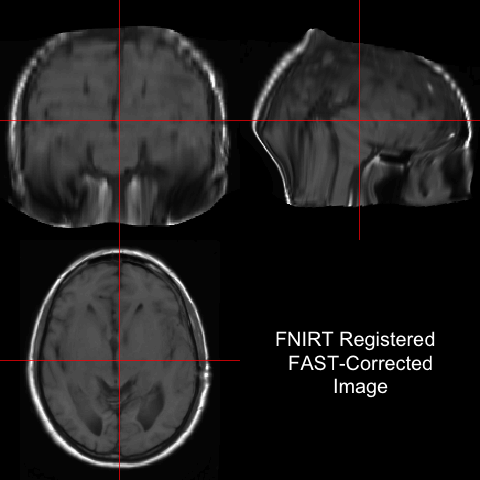
\includegraphics[width=0.5\linewidth]{FNIRT_Reg_Image.png}
\end{tabular}

\end{frame}



\begin{frame}[t,allowframebreaks]
  \frametitle{References}
  \printbibliography
 \end{frame}
 
\end{document}
